% REMEMBER: You must not plagiarise anything in your report. Be extremely careful.

\documentclass{l4proj}
\usepackage{subfiles}
\usepackage{pdfpages}

    
%
% put any additional packages here
%

\begin{document}

%==============================================================================
%% METADATA
\title{RViT - A Requirement and Value Identification Tool for Prioritisation}
\author{Niamh Gillespie}
\date{March 22, 2024}

\maketitle

%==============================================================================
%% ABSTRACT
\begin{abstract}
    Current agile project management tooling approaches are either feature-rich implementations which come with considerable administrative, complexity, and financial overheads or are overly simplified, drawing on few areas of agile methodology. RViT finds a middle ground between these two types of tools by providing an agile feature set designed to streamline the project management approach. The use of business values is also at the forefront of the tool with the goal of enhancing developer awareness of these values by increasing their visibility.

    Software developers were recruited to participant in a comprehensive user evaluation of RViT, with 56$\%$ of the study respondents stating that they found RViT easier to use or more intuitive than the industry leading tool Jira. Evaluations were also carried out to look into testing, performance and security and the results of these were deemed acceptable.
\end{abstract}

%==============================================================================

\chapter*{Acknowledgements}

I would like to thank my supervisor, Peggy Gregory, for her continued help and support throughout the duration of the project. I would also like to thank the developers who took part in my pilot study and user evaluation, their feedback was invaluable.

I also want to express my gratitude to my family and friends for putting up with me talking about RViT 24-7.

%==============================================================================
% EDUCATION REUSE CONSENT FORM
% If you consent to your project being shown to future students for educational purposes
% then insert your name and the date below to  sign the education use form that appears in the front of the document. 
% You must explicitly give consent if you wish to do so.
% If you sign, your project may be included in the Hall of Fame if it scores particularly highly.
%
% Please note that you are under no obligation to sign 
% this declaration, but doing so would help future students.
%
\def\consentname {Niamh Gillespie} % your full name
\def\consentdate {22 March 2024} % the date you agree
%
\educationalconsent


%==============================================================================
\tableofcontents

%==============================================================================
%% Notes on formatting
%==============================================================================
% The first page, abstract and table of contents are numbered using Roman numerals and are not
% included in the page count. 
%
% From now on pages are numbered
% using Arabic numerals. Therefore, immediately after the first call to \chapter we need the call
% \pagenumbering{arabic} and this should be called once only in the document. 
%
% Do not alter the bibliography style.
%
% The first Chapter should then be on page 1. You are allowed 40 pages for a 40 credit project and 30 pages for a 
% 20 credit report. This includes everything numbered in Arabic numerals (excluding front matter) up
% to but excluding the appendices and bibliography.
%
% You must not alter text size (it is currently 10pt) or alter margins or spacing.
%
%
%==================================================================================================================================
%
% IMPORTANT
% The chapter headings here are **suggestions**. You don't have to follow this model if
% it doesn't fit your project. Every project should have an introduction and conclusion,
% however. 
%
%==================================================================================================================================
\chapter{Introduction}

% reset page numbering. Don't remove this!
\pagenumbering{arabic} 

\subfile{Introduction}


%==================================================================================================================================
\chapter{Background}
\subfile{Background}
%==================================================================================================================================
\chapter{Requirement Analysis}
\subfile{Requirements}

%==================================================================================================================================
\chapter{Design}
\subfile{Design}

%==================================================================================================================================
\chapter{Implementation}
\subfile{Implementation}

%==================================================================================================================================
\chapter{Evaluation} 
\subfile{Evaluation}
%==================================================================================================================================
\chapter{Conclusion}    
\subfile{Conclusion}

%==================================================================================================================================
%
% 
%==================================================================================================================================
%  APPENDICES  

\begin{appendices}

\chapter{Database Schema}
\label{app: database}

\centerline{
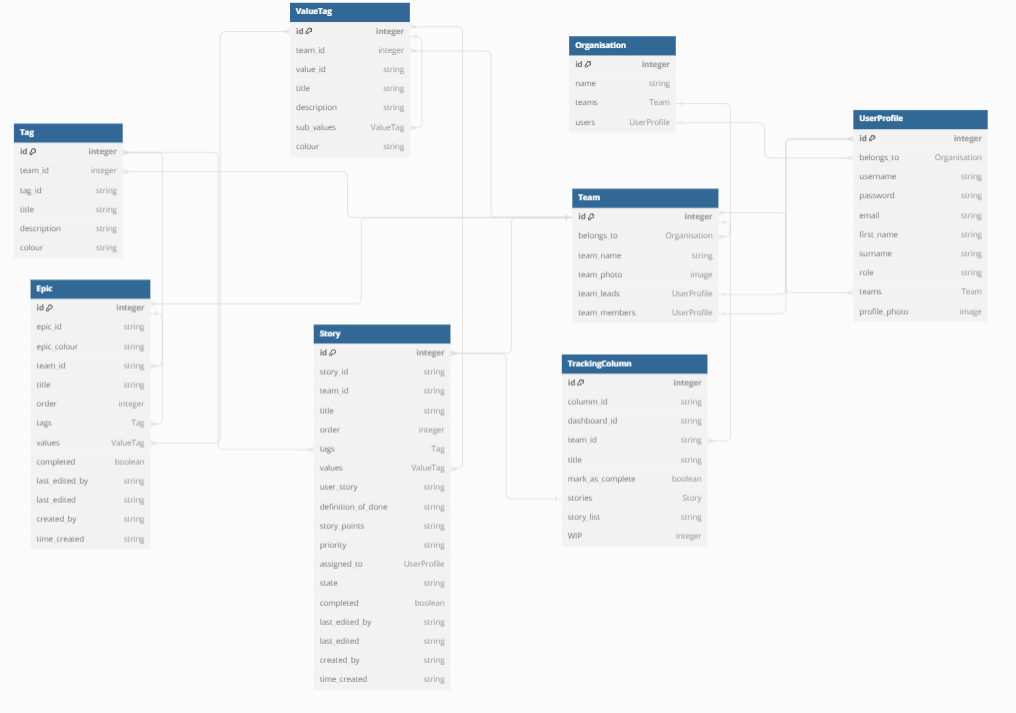
\includegraphics[width=1.2\textwidth, page=1]{dissertation/appendices/DatabaseDiagram.png}
}

\chapter{Enlarged epic and user story detail modals}
\label{app: epics and us details}

\begin{figure}[h!]
\centering
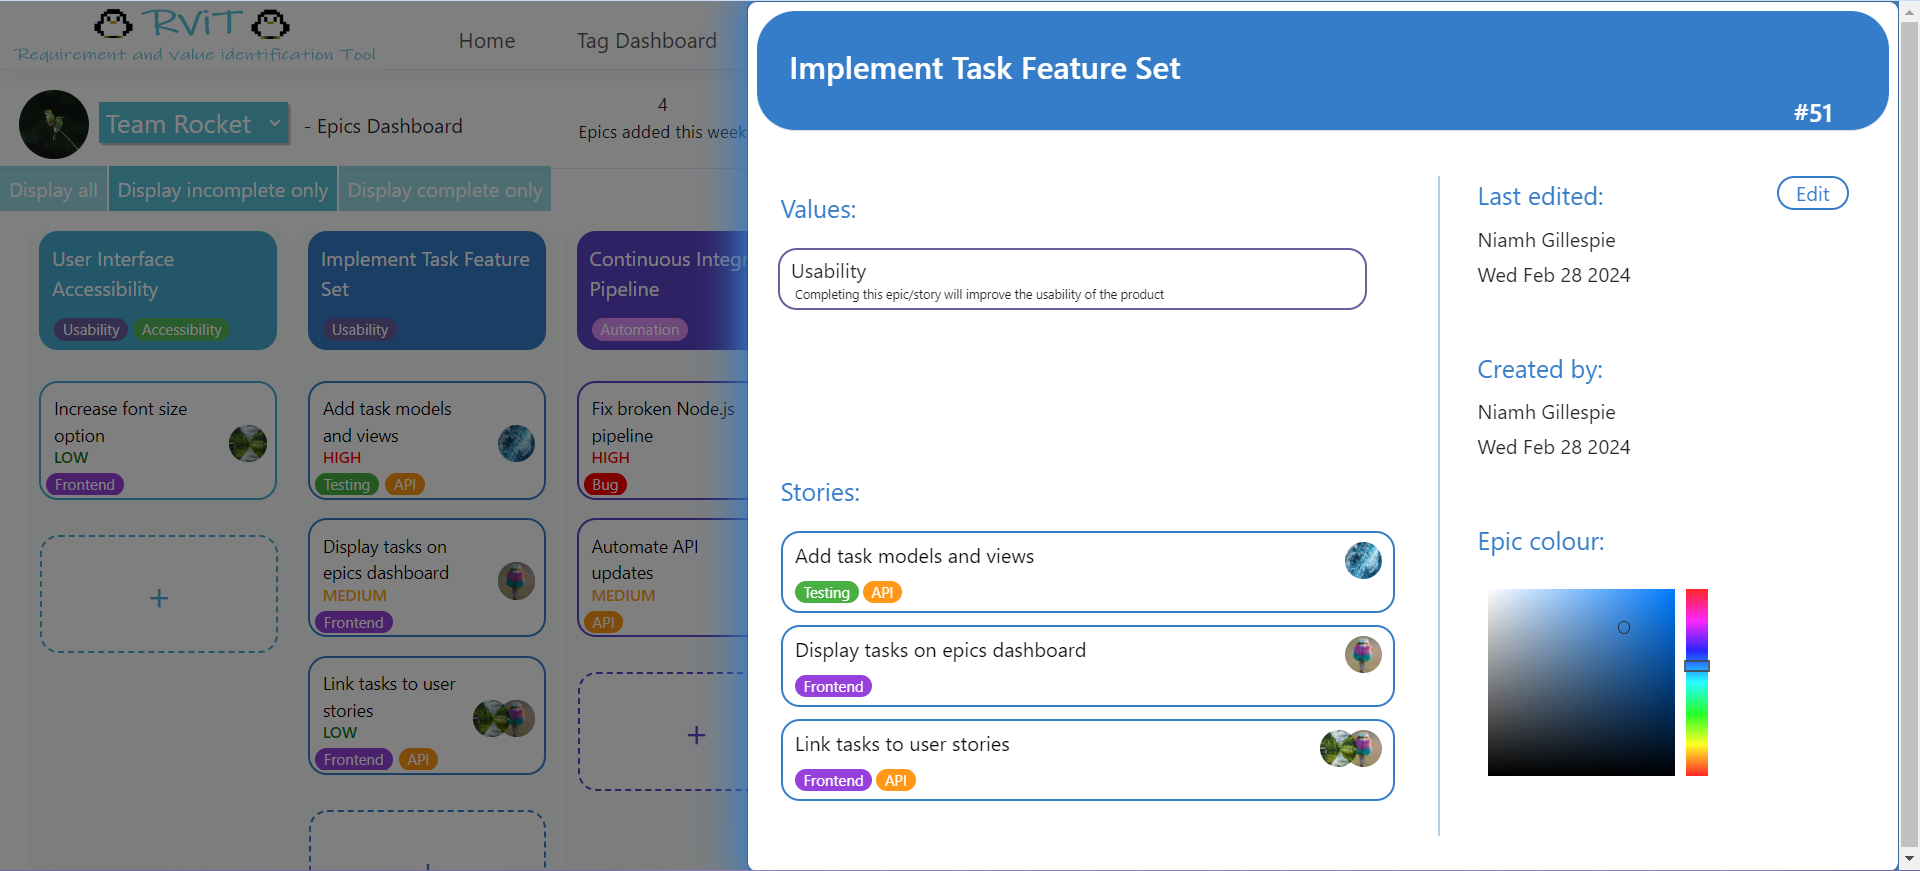
\includegraphics[scale=0.4]{dissertation/images/EpicDetails.png}
\caption{Large Epic details modal}
\label{fig: large epic detail modals}
\end{figure}
\hfill
\begin{figure}[h!]
\centering
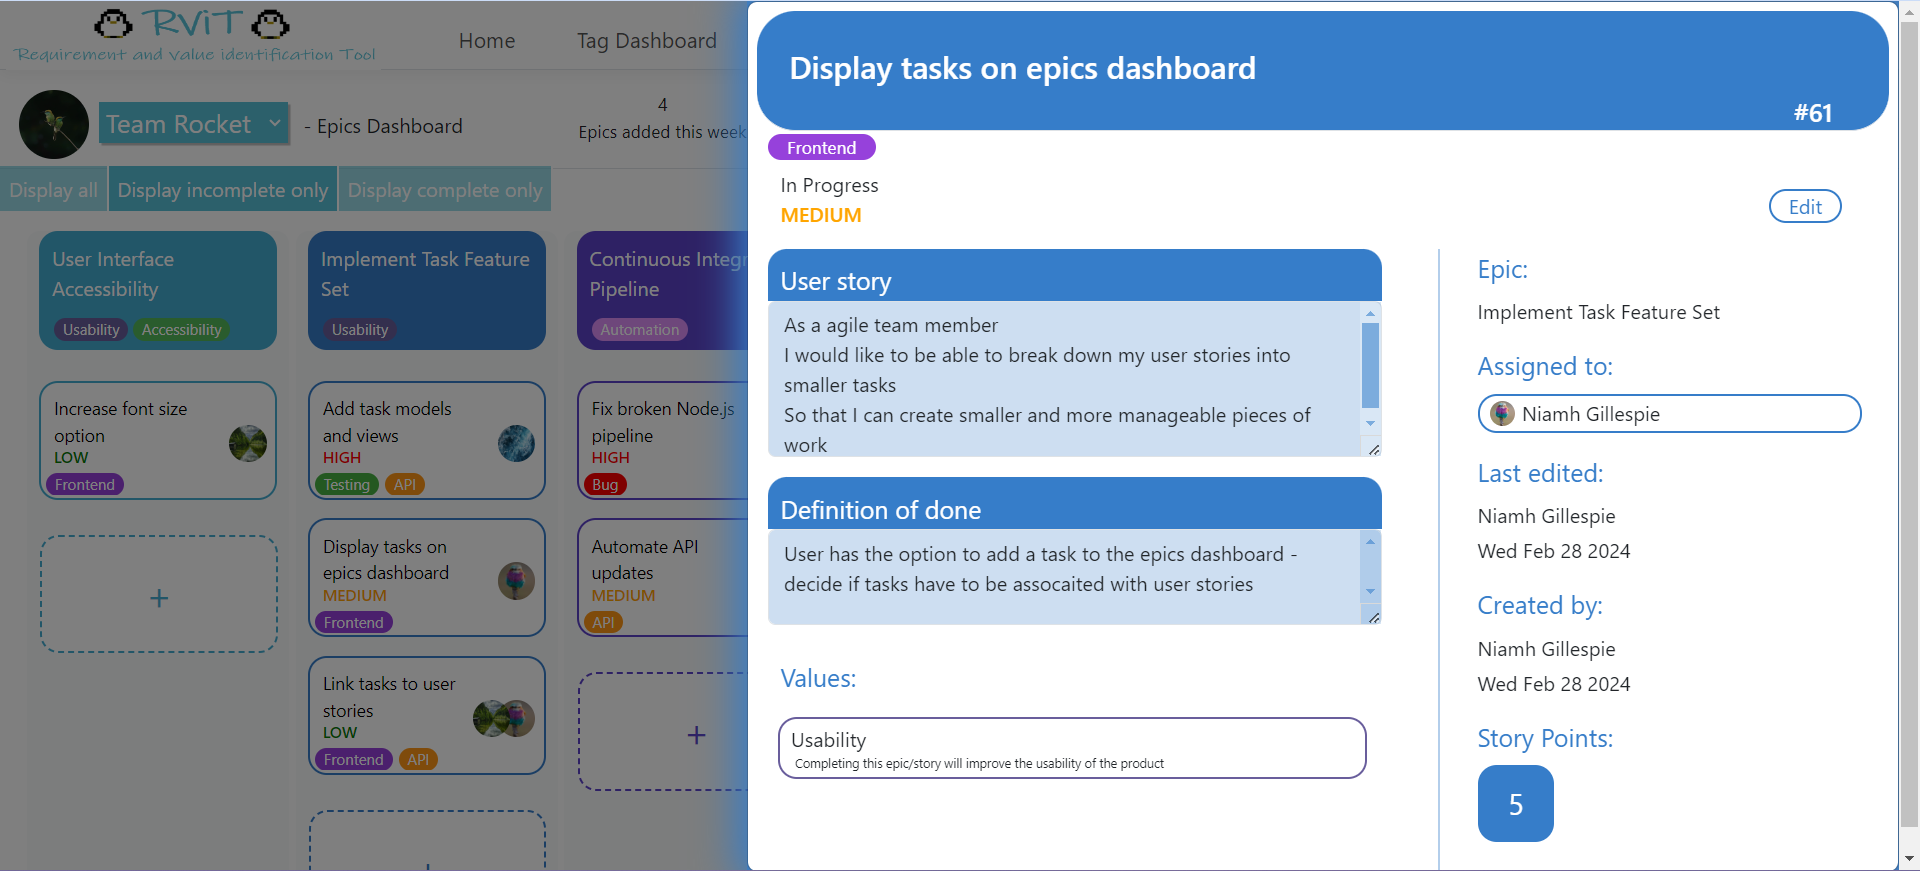
\includegraphics[scale=0.4]{dissertation/images/StoryDetails.png}
\caption{Large Story details modal}
\label{fig:large story detail modals}
\end{figure}

\chapter{Enlarged Tag Dashboard pages}
\label{app: large tag and value views}

\begin{figure}[h!]
\centering
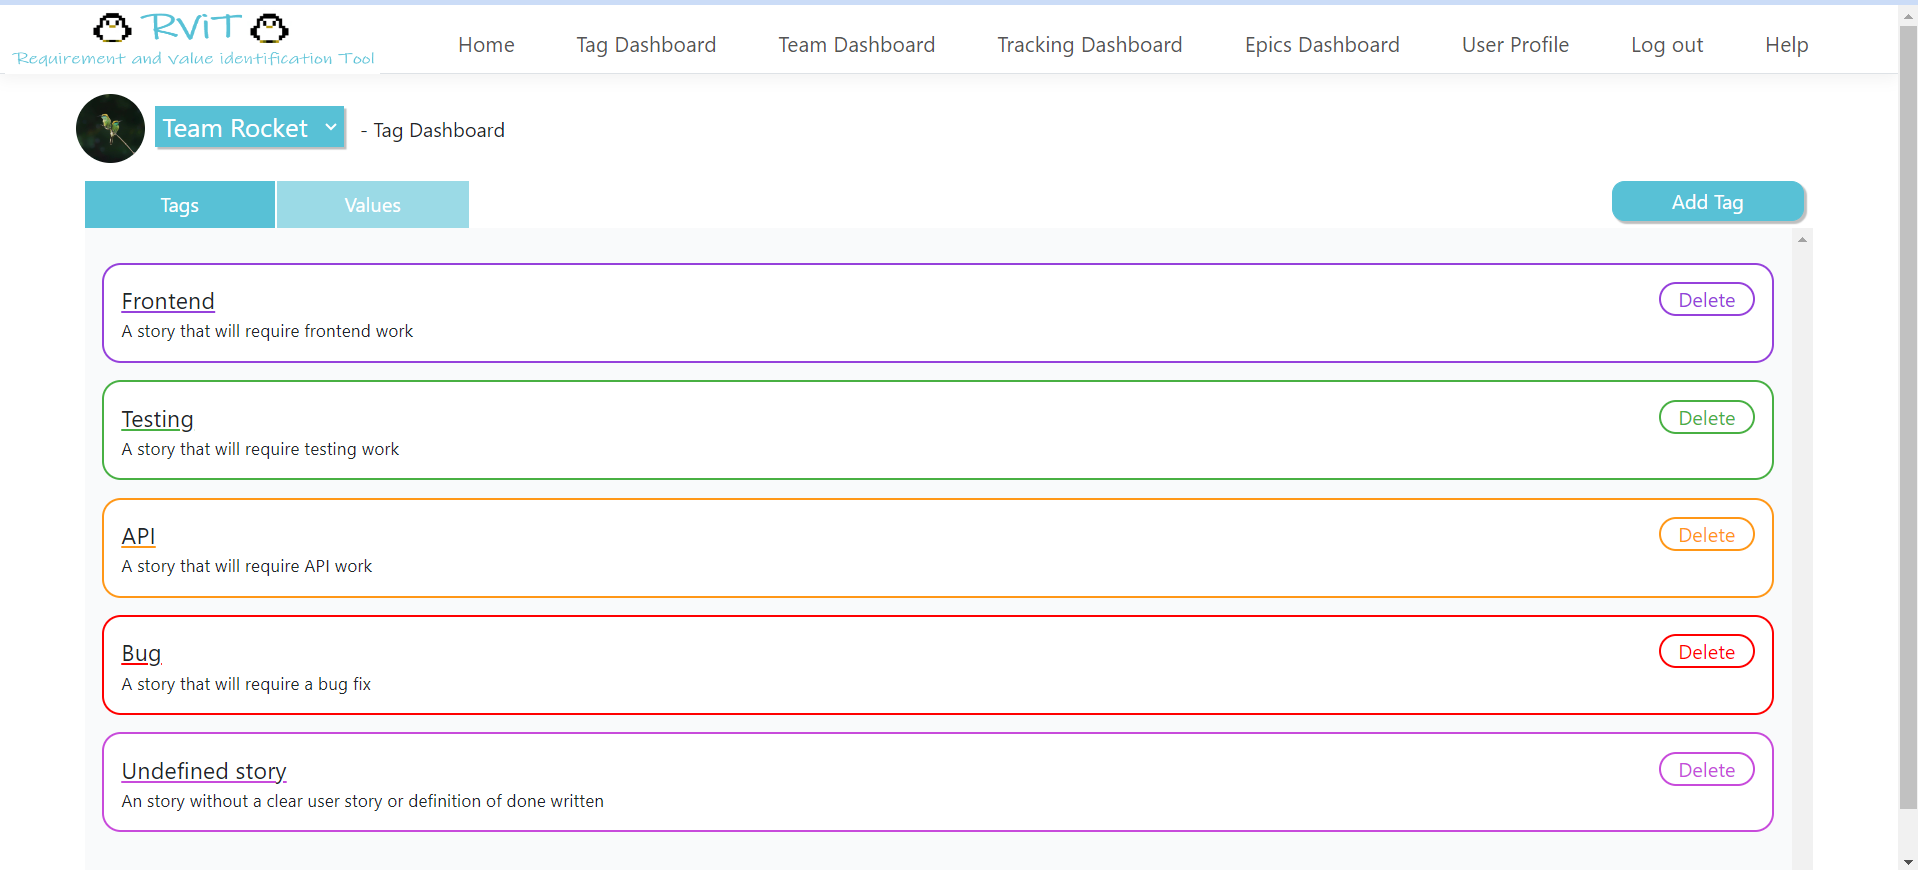
\includegraphics[scale=0.4]{dissertation/images/TagDashboardOne.png}
\caption{Large Tag dashboard - tag overview}
\label{fig: large tag dashboard - tag overview}
\end{figure}
\hfill
\begin{figure}[h!]
\centering
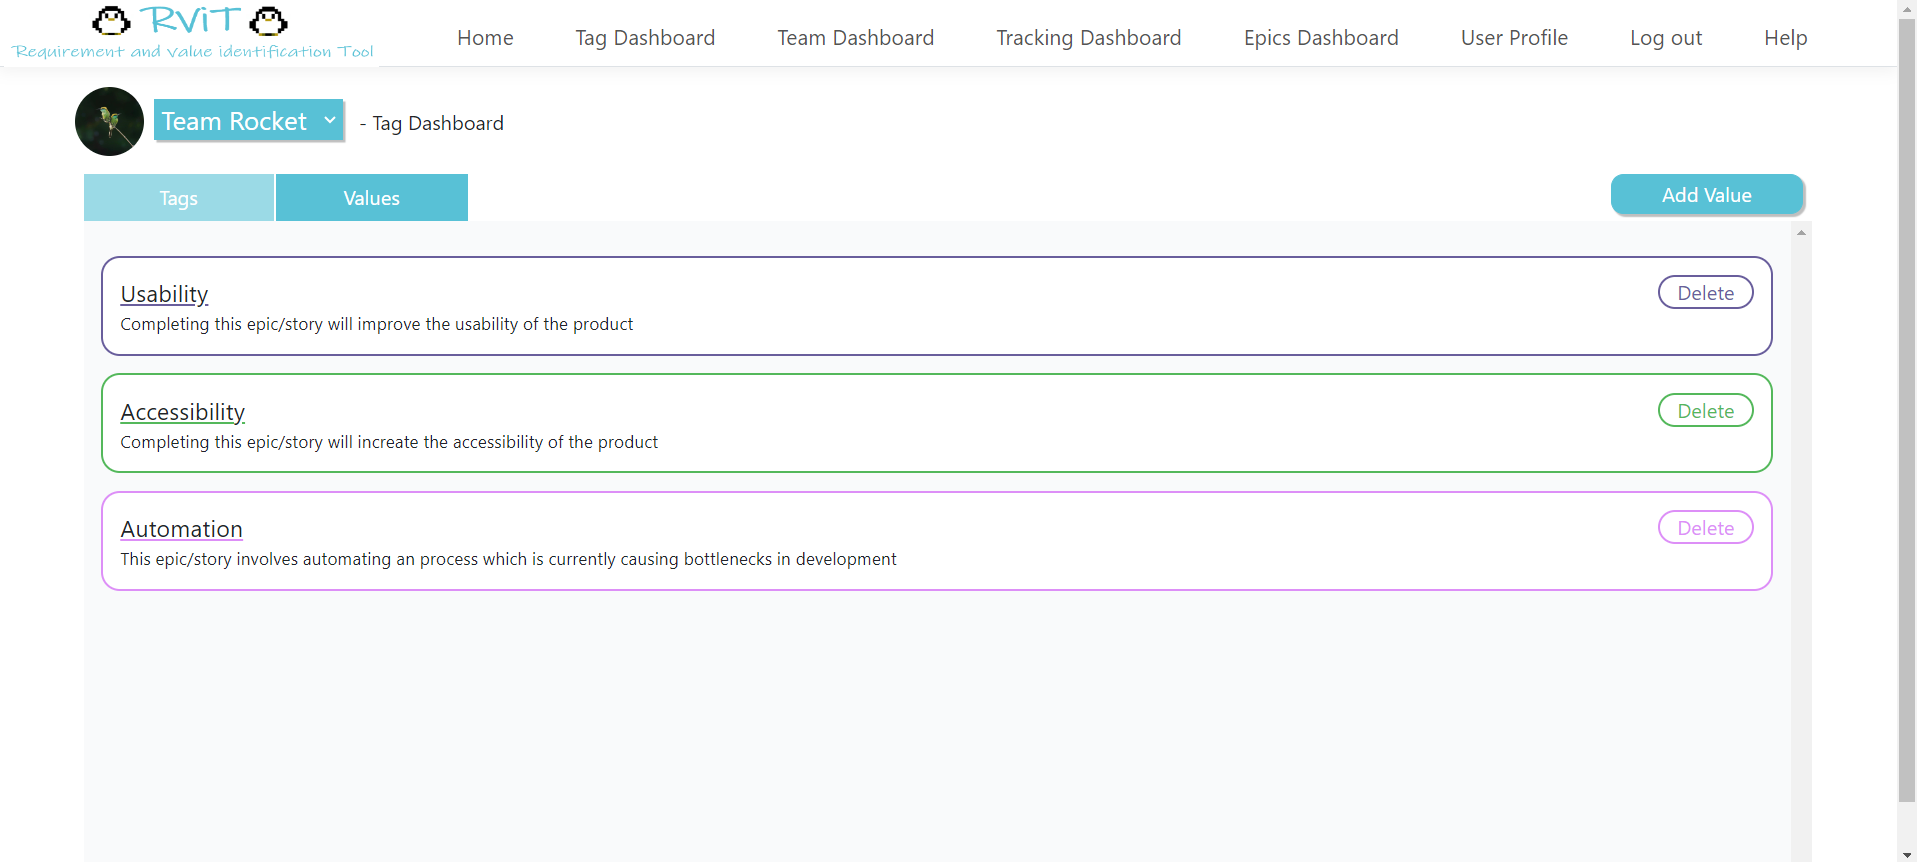
\includegraphics[scale=0.4]{dissertation/images/TagDashboardTwo.png}
\caption{Tag dashboard - values overview}
\label{fig:large Tag dashboard - values overviews}
\end{figure}


\chapter{Admin workflow pages}
\label{app: admin workflow}

\begin{figure}[h!]
\centering
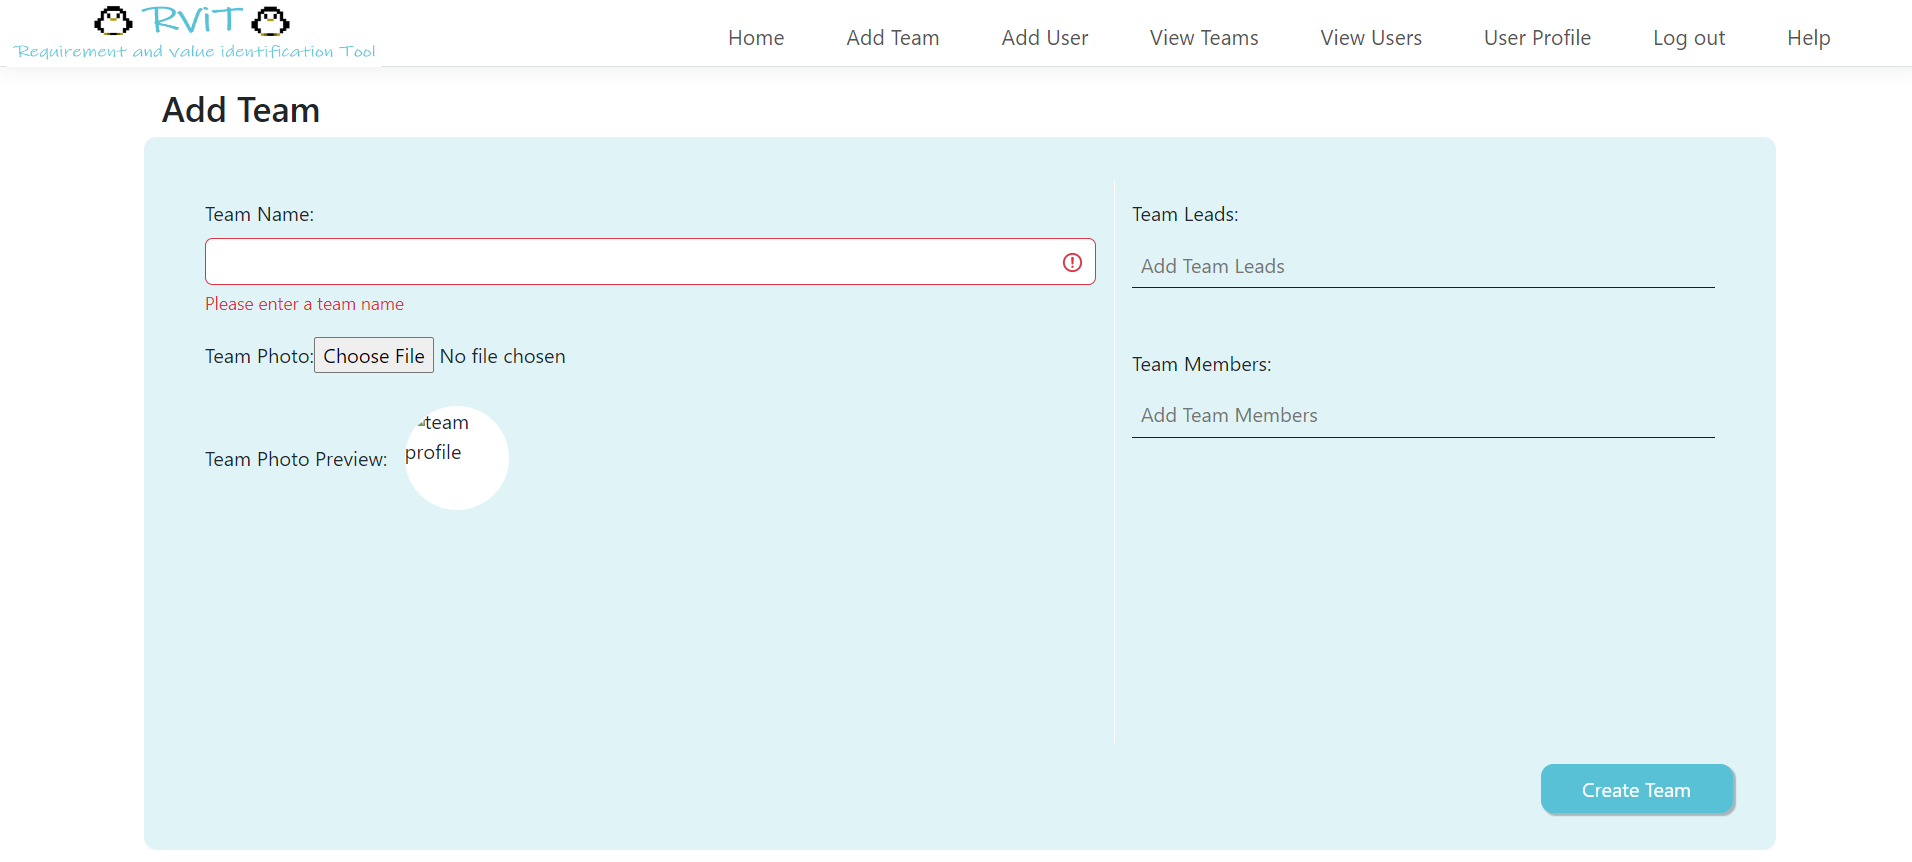
\includegraphics[scale=0.4]{dissertation/images/addteam.png}
\caption{Add team page}
\label{fig: add team page}
\end{figure}
\hfill
\begin{figure}[h!]
\centering
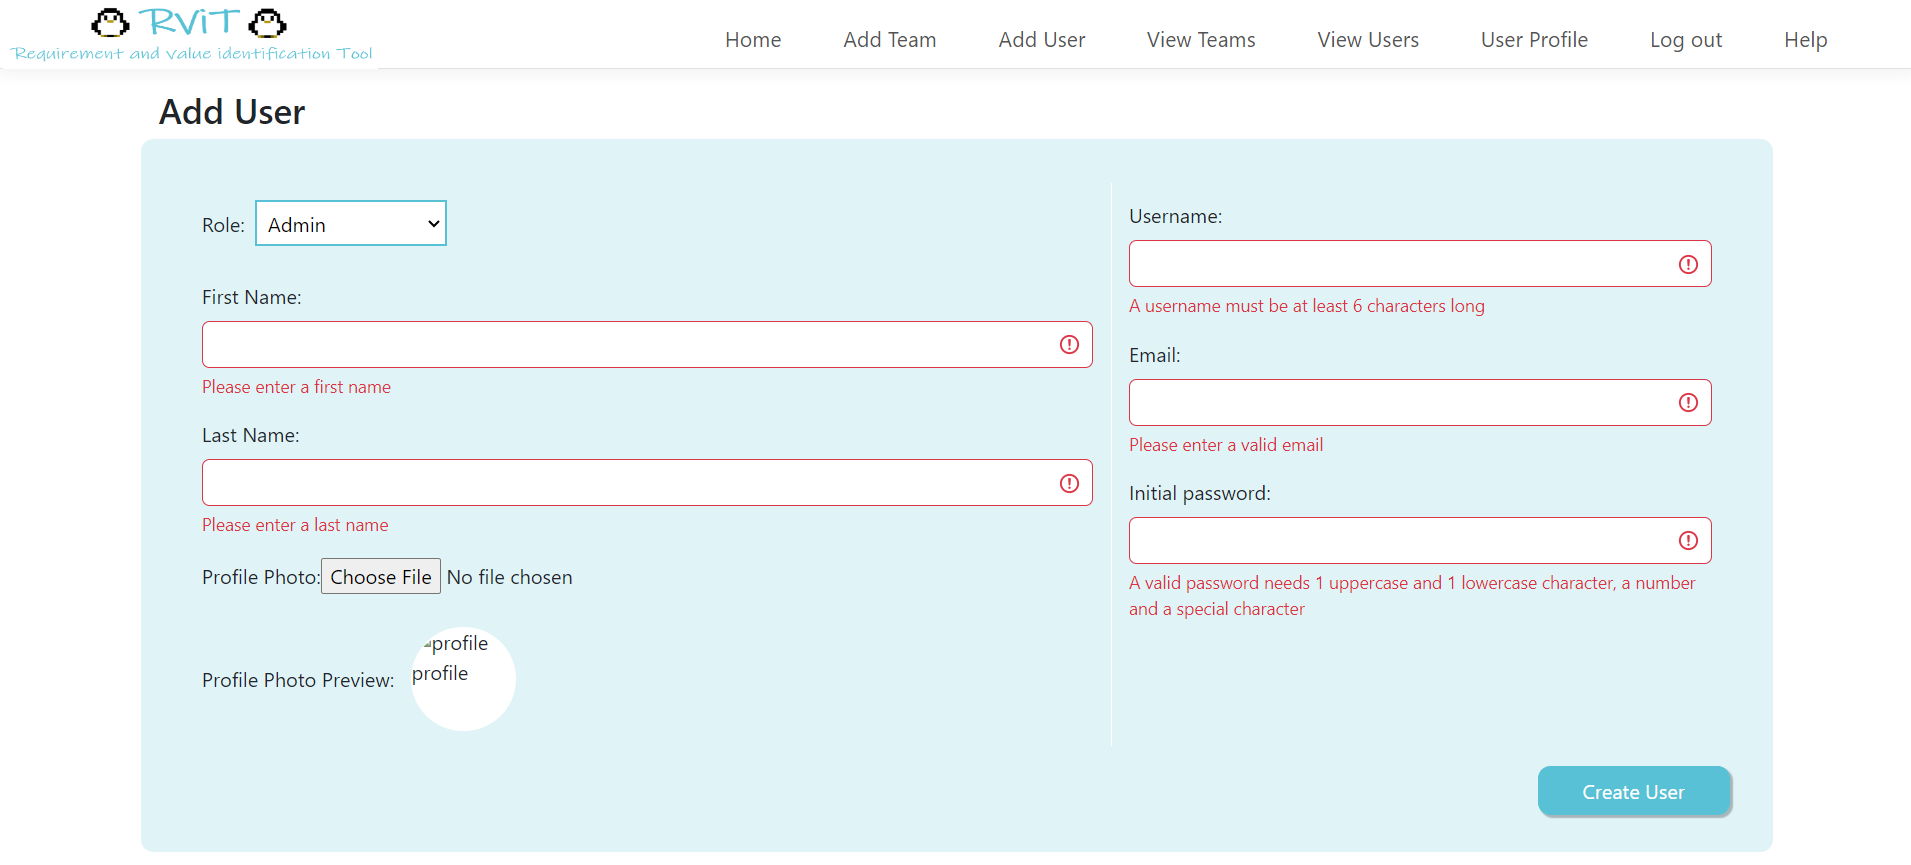
\includegraphics[scale=0.4]{dissertation/images/adduser.png}
\caption{Add user page}
\label{fig: add user page}
\end{figure}
\hfill
\begin{figure}[h!]
\centering
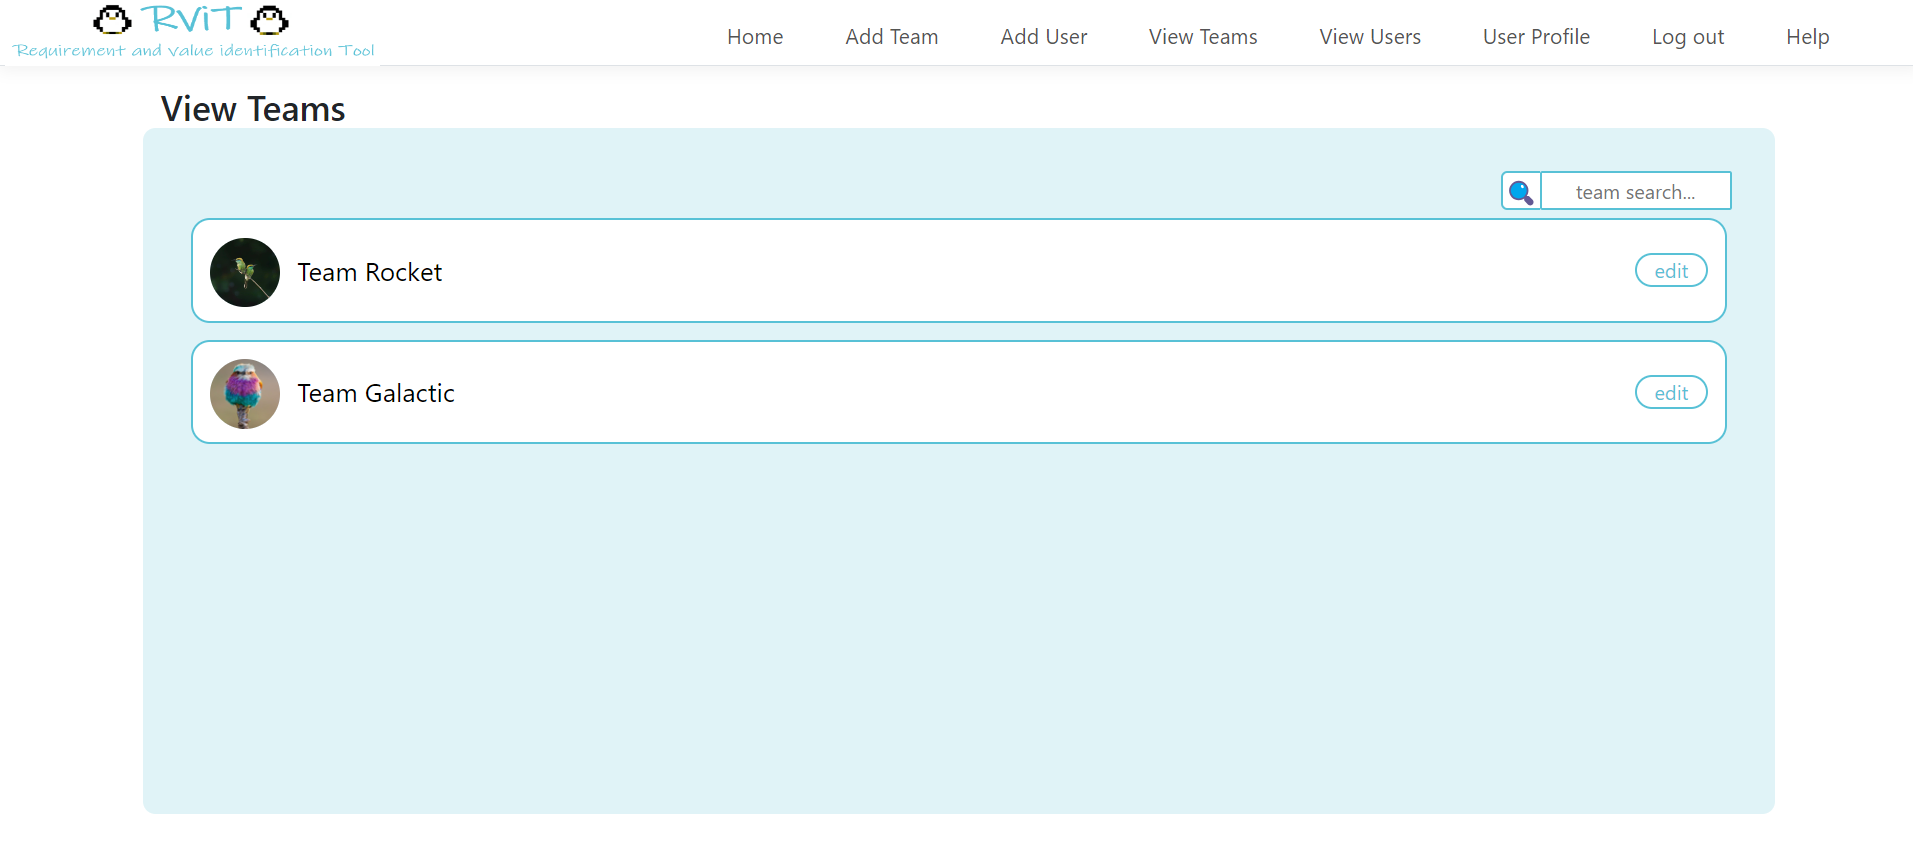
\includegraphics[scale=0.4]{dissertation/images/viewteams.png}
\caption{View Teams page}
\label{fig: view team page}
\end{figure}
\hfill
\begin{figure}[h!]
\centering
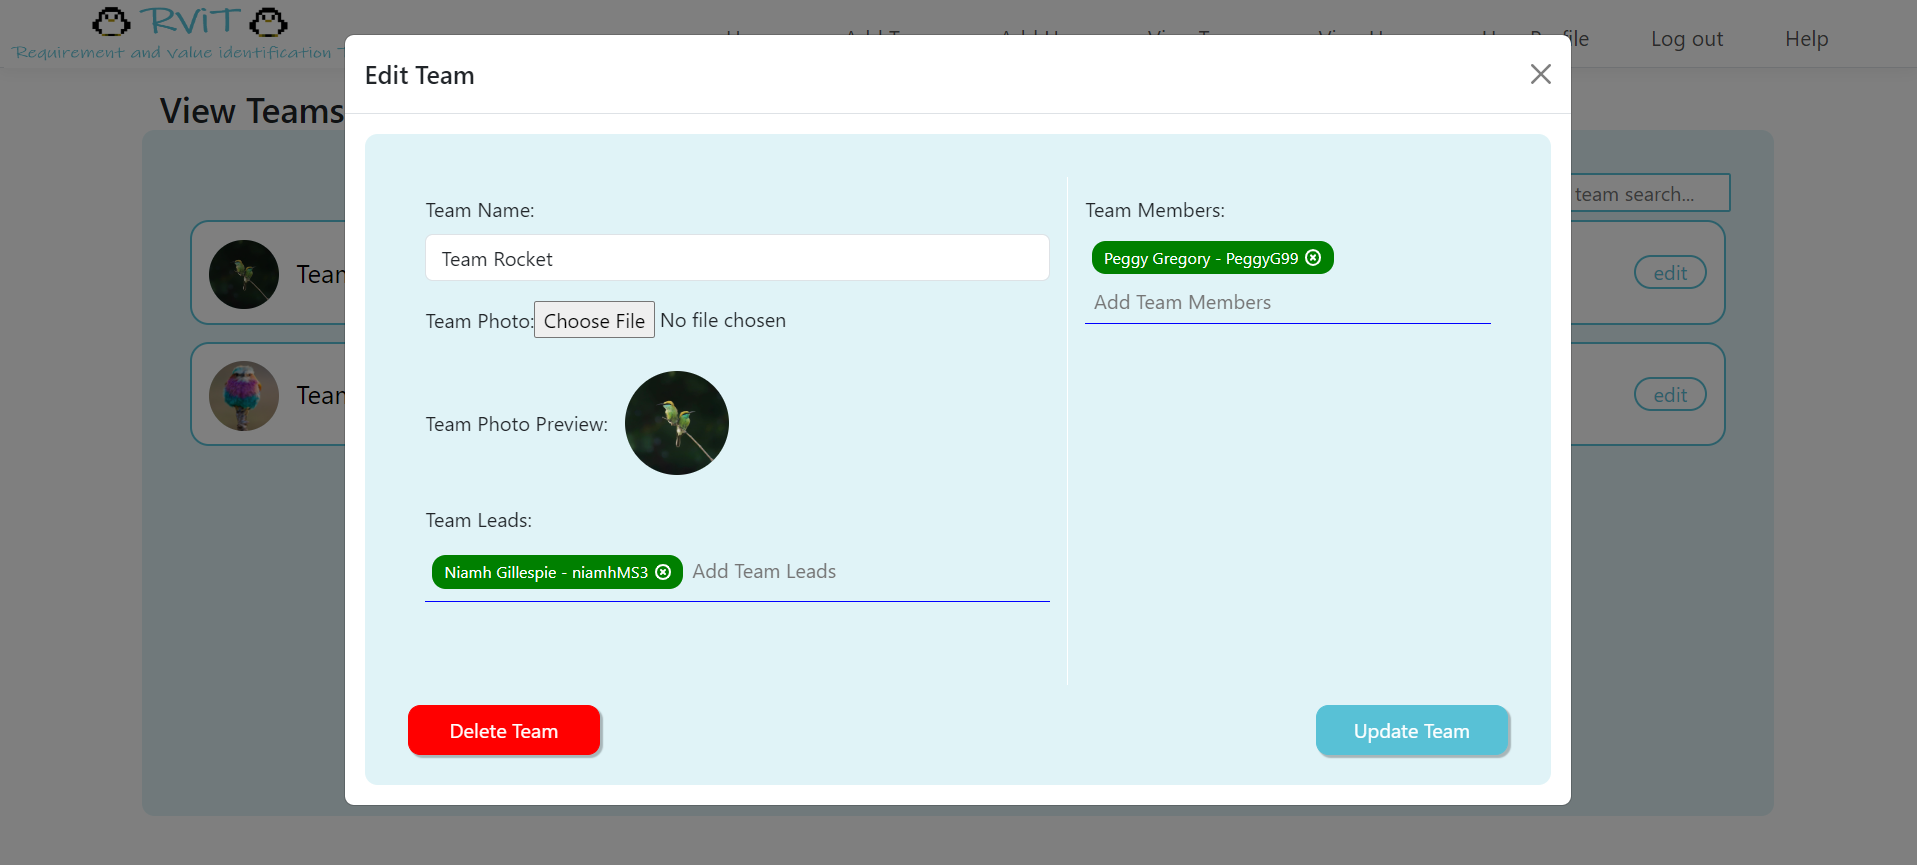
\includegraphics[scale=0.4]{dissertation/images/editteam.png}
\caption{Edit Team modal}
\label{fig: edit team modal}
\end{figure}
\hfill
\begin{figure}[h!]
\centering
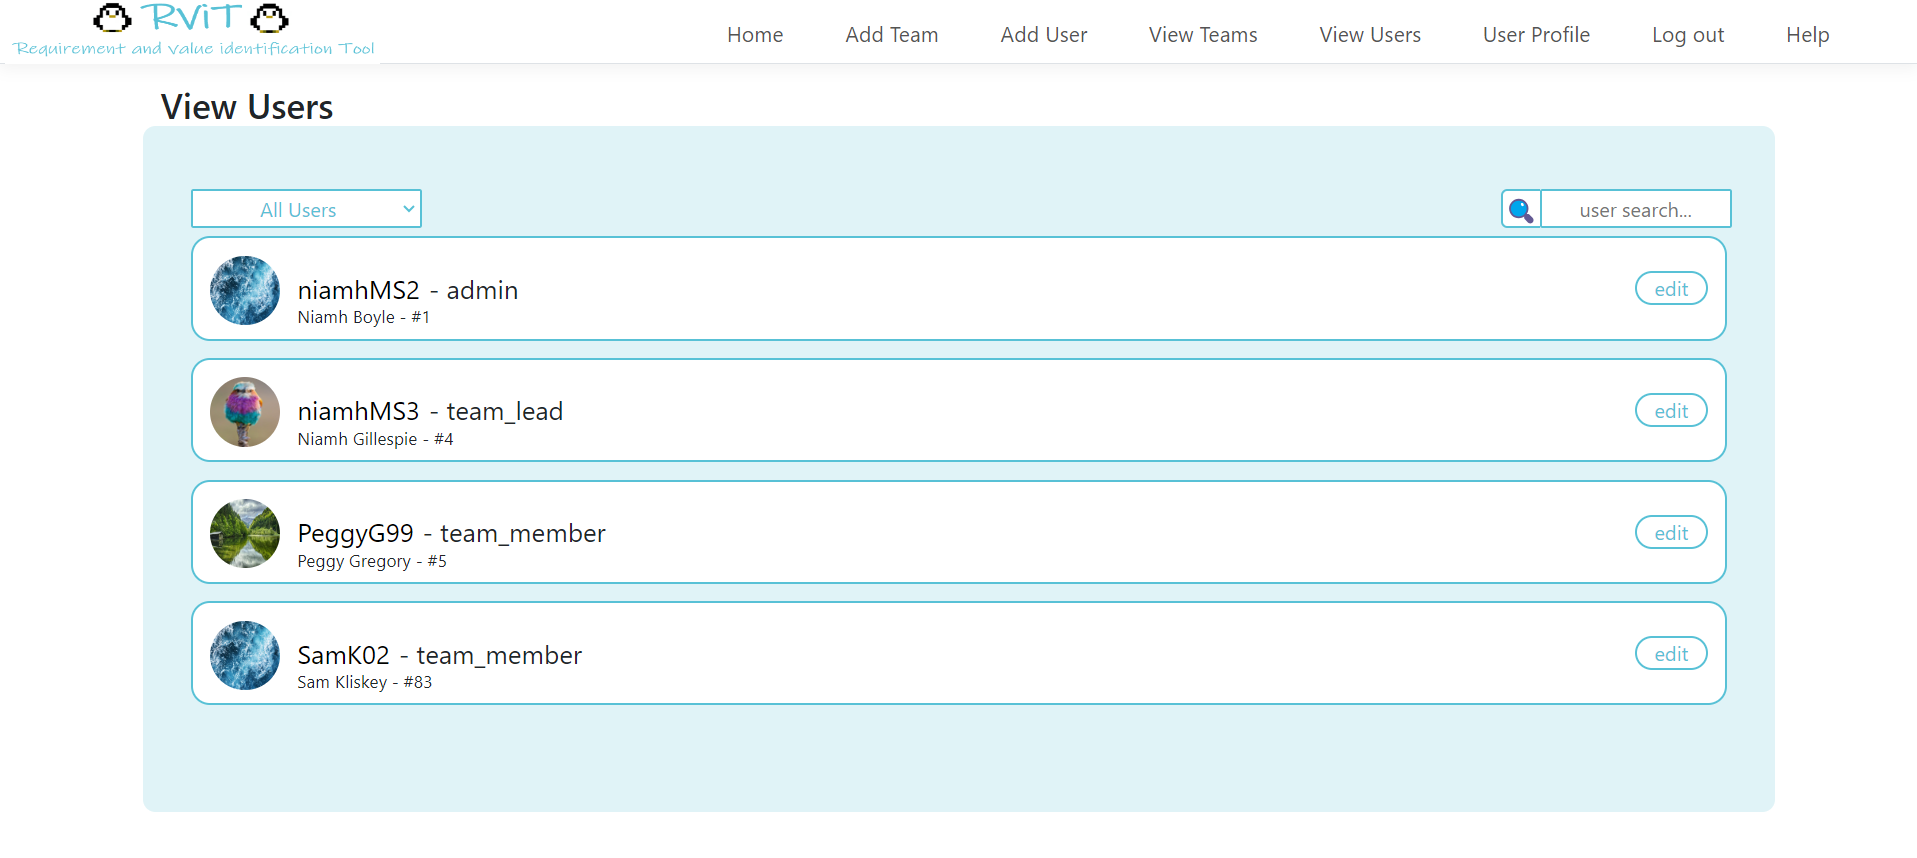
\includegraphics[scale=0.4]{dissertation/images/viewuser.png}
\caption{View Users page}
\label{fig: view user page}
\end{figure}
\hfill\begin{figure}[h!]
\centering
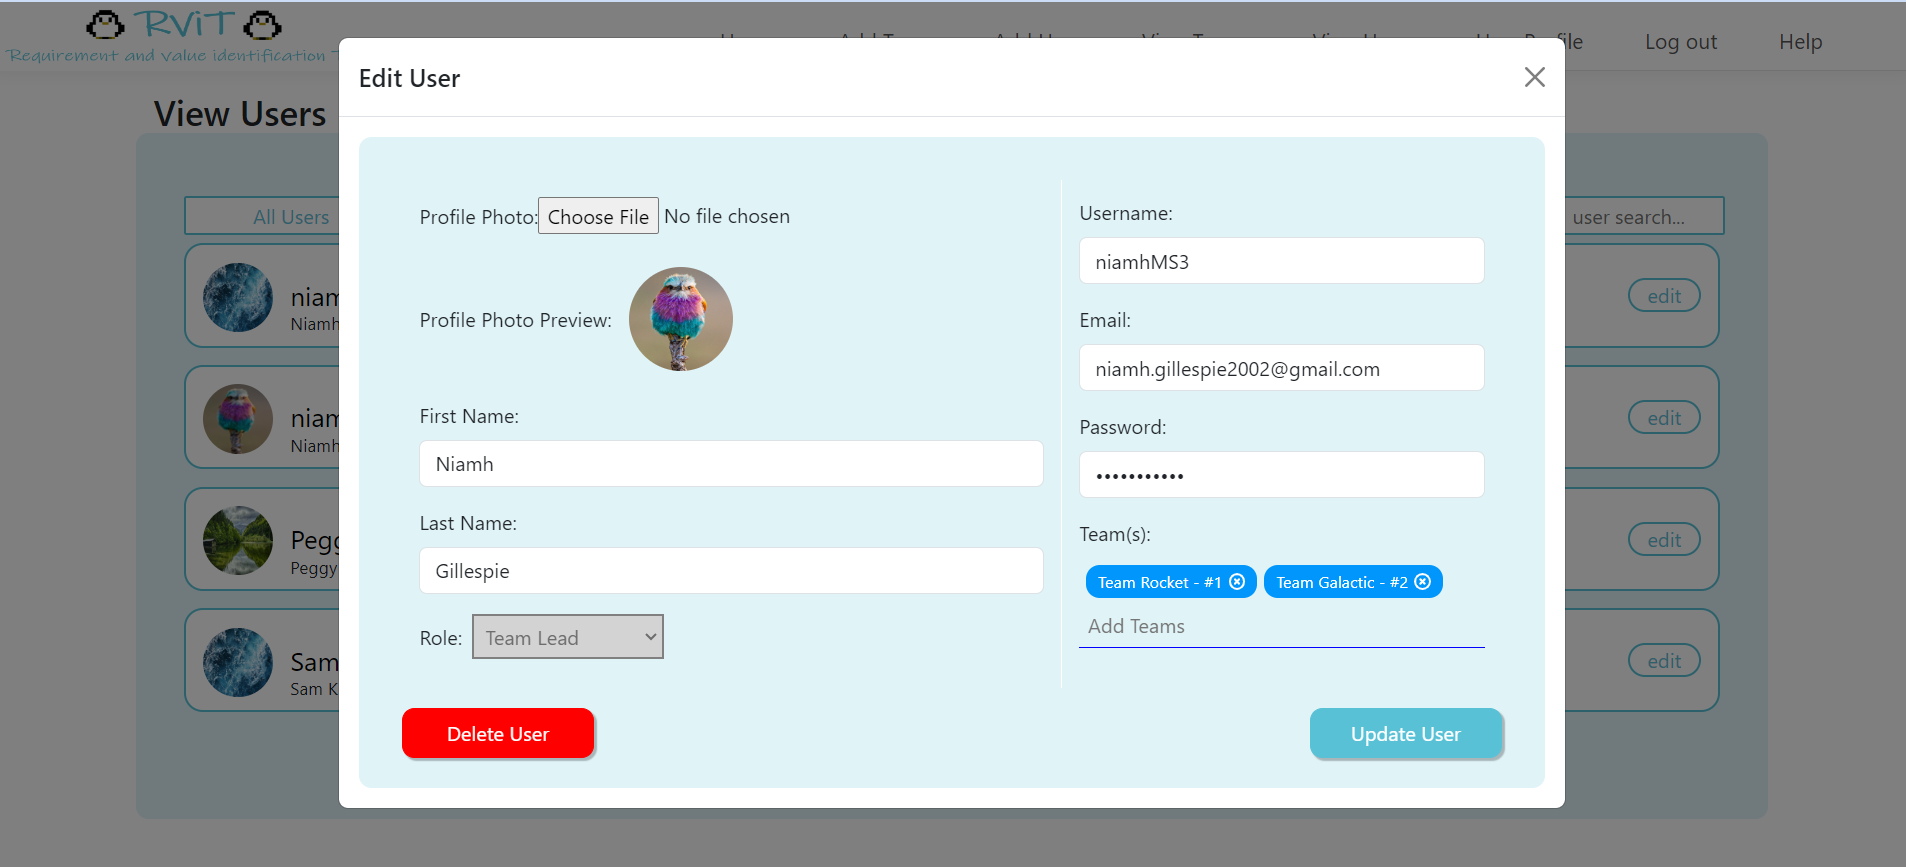
\includegraphics[scale=0.4]{dissertation/images/edituser.png}
\caption{Edit User modal}
\label{fig: edit user page}
\end{figure}




\chapter{User authentication pages}
\label{app: user authentication workflow}

\begin{figure}[h!]
\centering
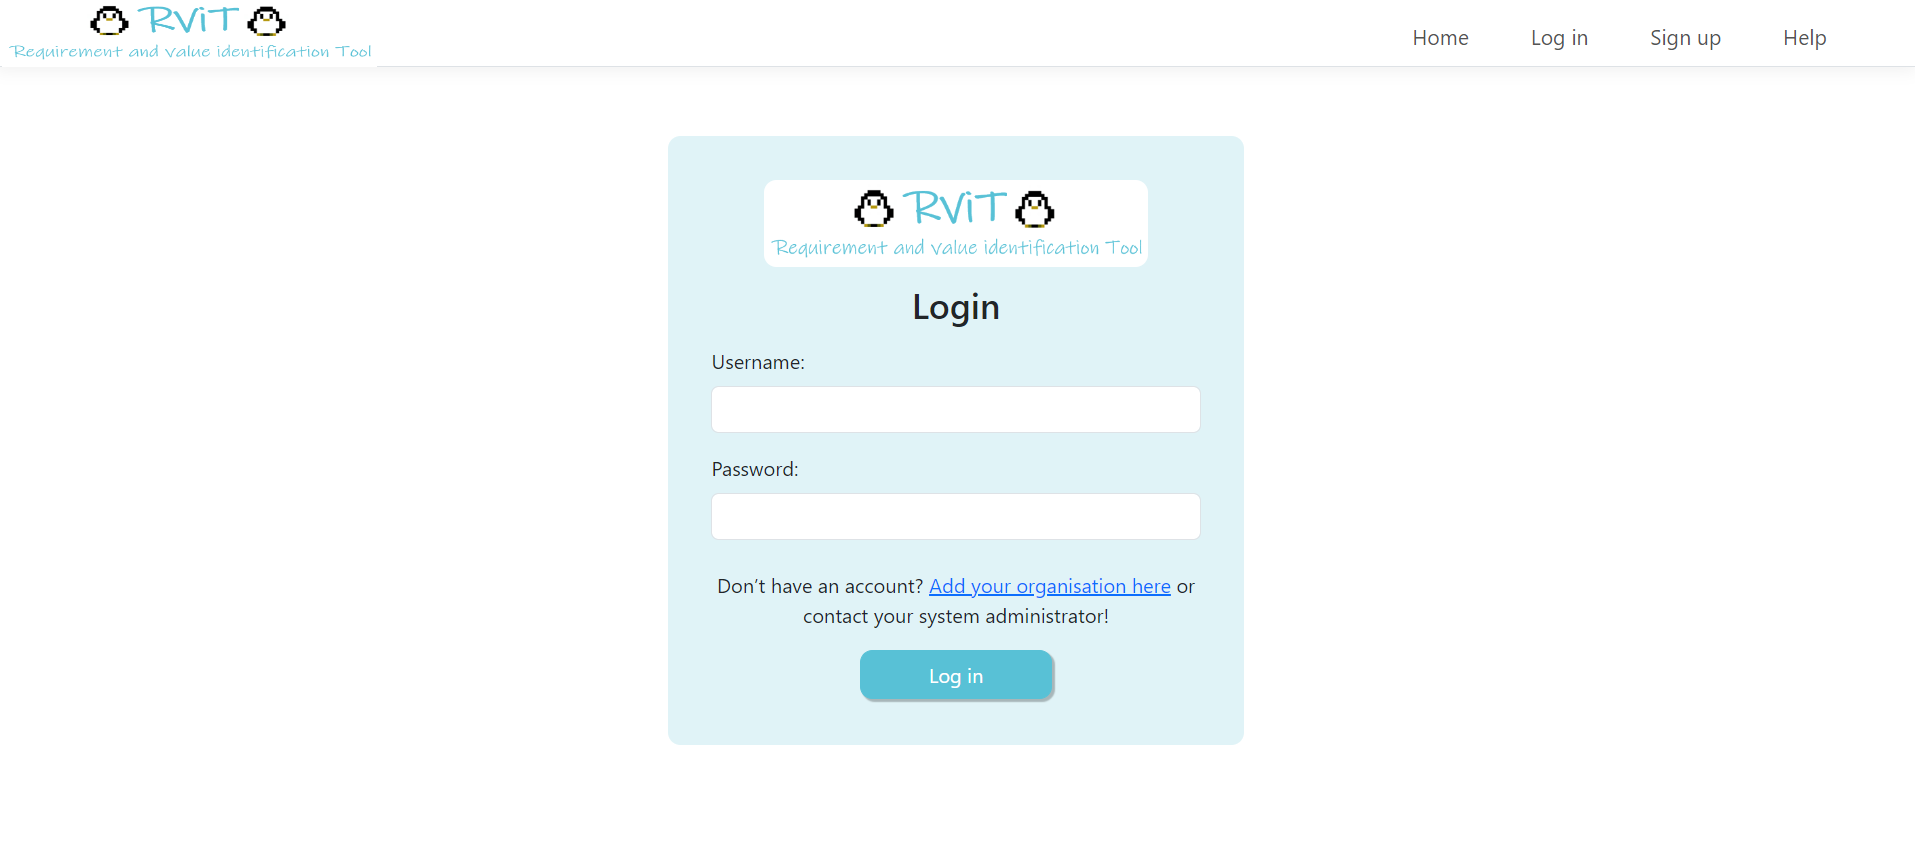
\includegraphics[scale=0.4]{dissertation/images/login.png}
\caption{Log-in page}
\label{fig: login}
\end{figure}
\hfill
\begin{figure}[h!]
\centering
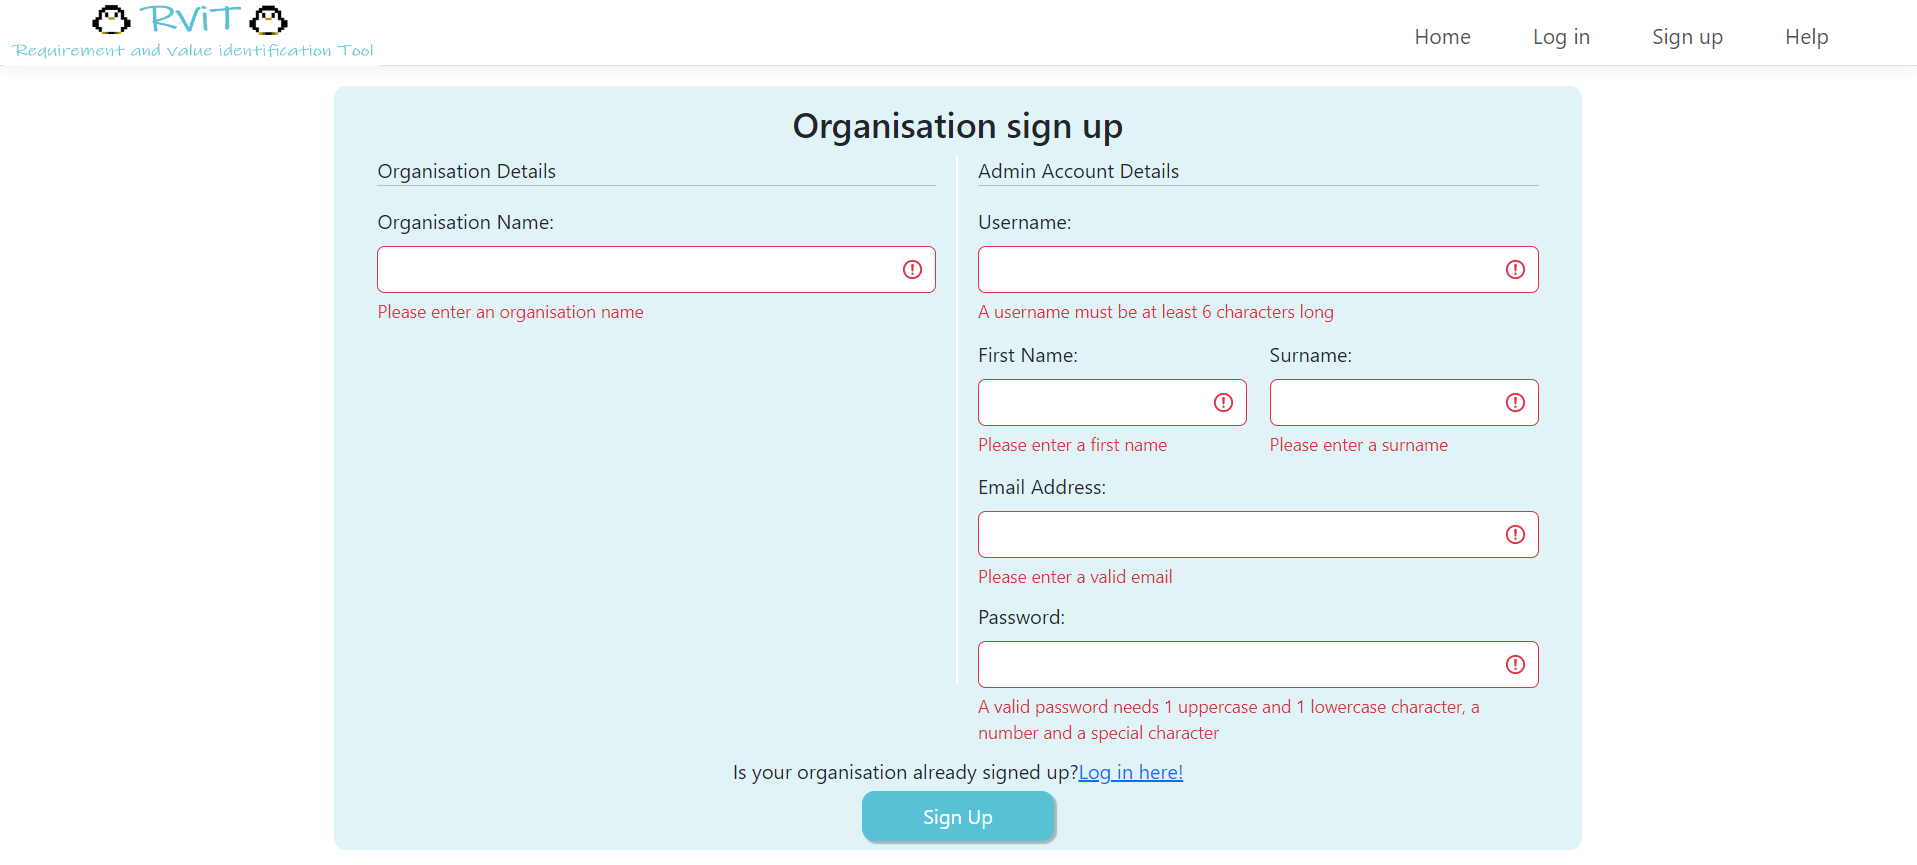
\includegraphics[scale=0.4]{dissertation/images/sign up.png}
\caption{Sign-up page}
\label{fig:sign up}
\end{figure}

\chapter{Ethics Checklist}
\label{app: ethics checklist}

\centerline{
\includegraphics[width=0.9\textwidth, pages={1}]{dissertation/appendices/2549880G_ethics_checklist.pdf}
}

\includepdf[width=1\textwidth, pages={2}]{appendices/2549880G_ethics_checklist.pdf}

\chapter{User Evaluation Survey}
\label{app: user eval survey}

\centerline{
\includegraphics[width=0.9\textwidth, pages={1}]{dissertation/appendices/UserEvaluationSurveyForm.pdf}
}

\includepdf[width=1.2\textwidth, pages={2-5}]{appendices/UserEvaluationSurveyForm.pdf}


\chapter{Qualitative Coding of Text Responses from User Evaluation}
\label{app: qualitative coding}
\\
\centerline{
\includegraphics[width=0.85\textwidth, page=1]{dissertation/appendices/Qualitative coding of text responses.pdf}
}

\includepdf[width=1.2\textwidth, pages={2-10}]{appendices/Qualitative coding of text responses.pdf}

\end{appendices}

%==================================================================================================================================
%   BIBLIOGRAPHY   

% The bibliography style is abbrvnat
% The bibliography always appears last, after the appendices.

\bibliographystyle{abbrvnat}

\bibliography{l4proj}

\end{document}
